\documentclass{beamer}

\usetheme{JKI}

\usepackage[english]{babel}

\usepackage{hyperref,multirow,natbib,grffile}
\hypersetup{
	%pdfpagemode = FullScreen,
	%pdfpagetransition = Wipe
}
%change if you like
\setboolean{firstBlack}{false} 
\renewcommand{\InstLogo}{JKI_logo_german.pdf}

\title{Die Bedeutung von \textit{Feature Engineering} bei der KI-basierten räumlichen Modellierung am Beispiel einer DSM-Anwendung}

\author{Markus Möller$^1$, Simone Zepp$^{2}$, Martin Wiesmeier$^{3}$, Heike Gerighausen$^{1}$ und Uta Heiden$^{2}$}


\institute{
\vspace{5pt}\\
$^1$ Julius Kühn-Institut\\
$^2$ Deutsches Zentrum für Luft- und Raumfahrt e.V. (DLR)\\
$^3$ Bayrische Landesanstalt für Landwirtschaft (LfL)\\}



\renewcommand{\email}{KIDA-Fachtagung}
\begin{document}
\maketitle

\begin{frame}{Motivation}
\begin{block}{Exkursion zur DBG-Jahrestagung am 8.9.2023 (Eickendorf)}
\centering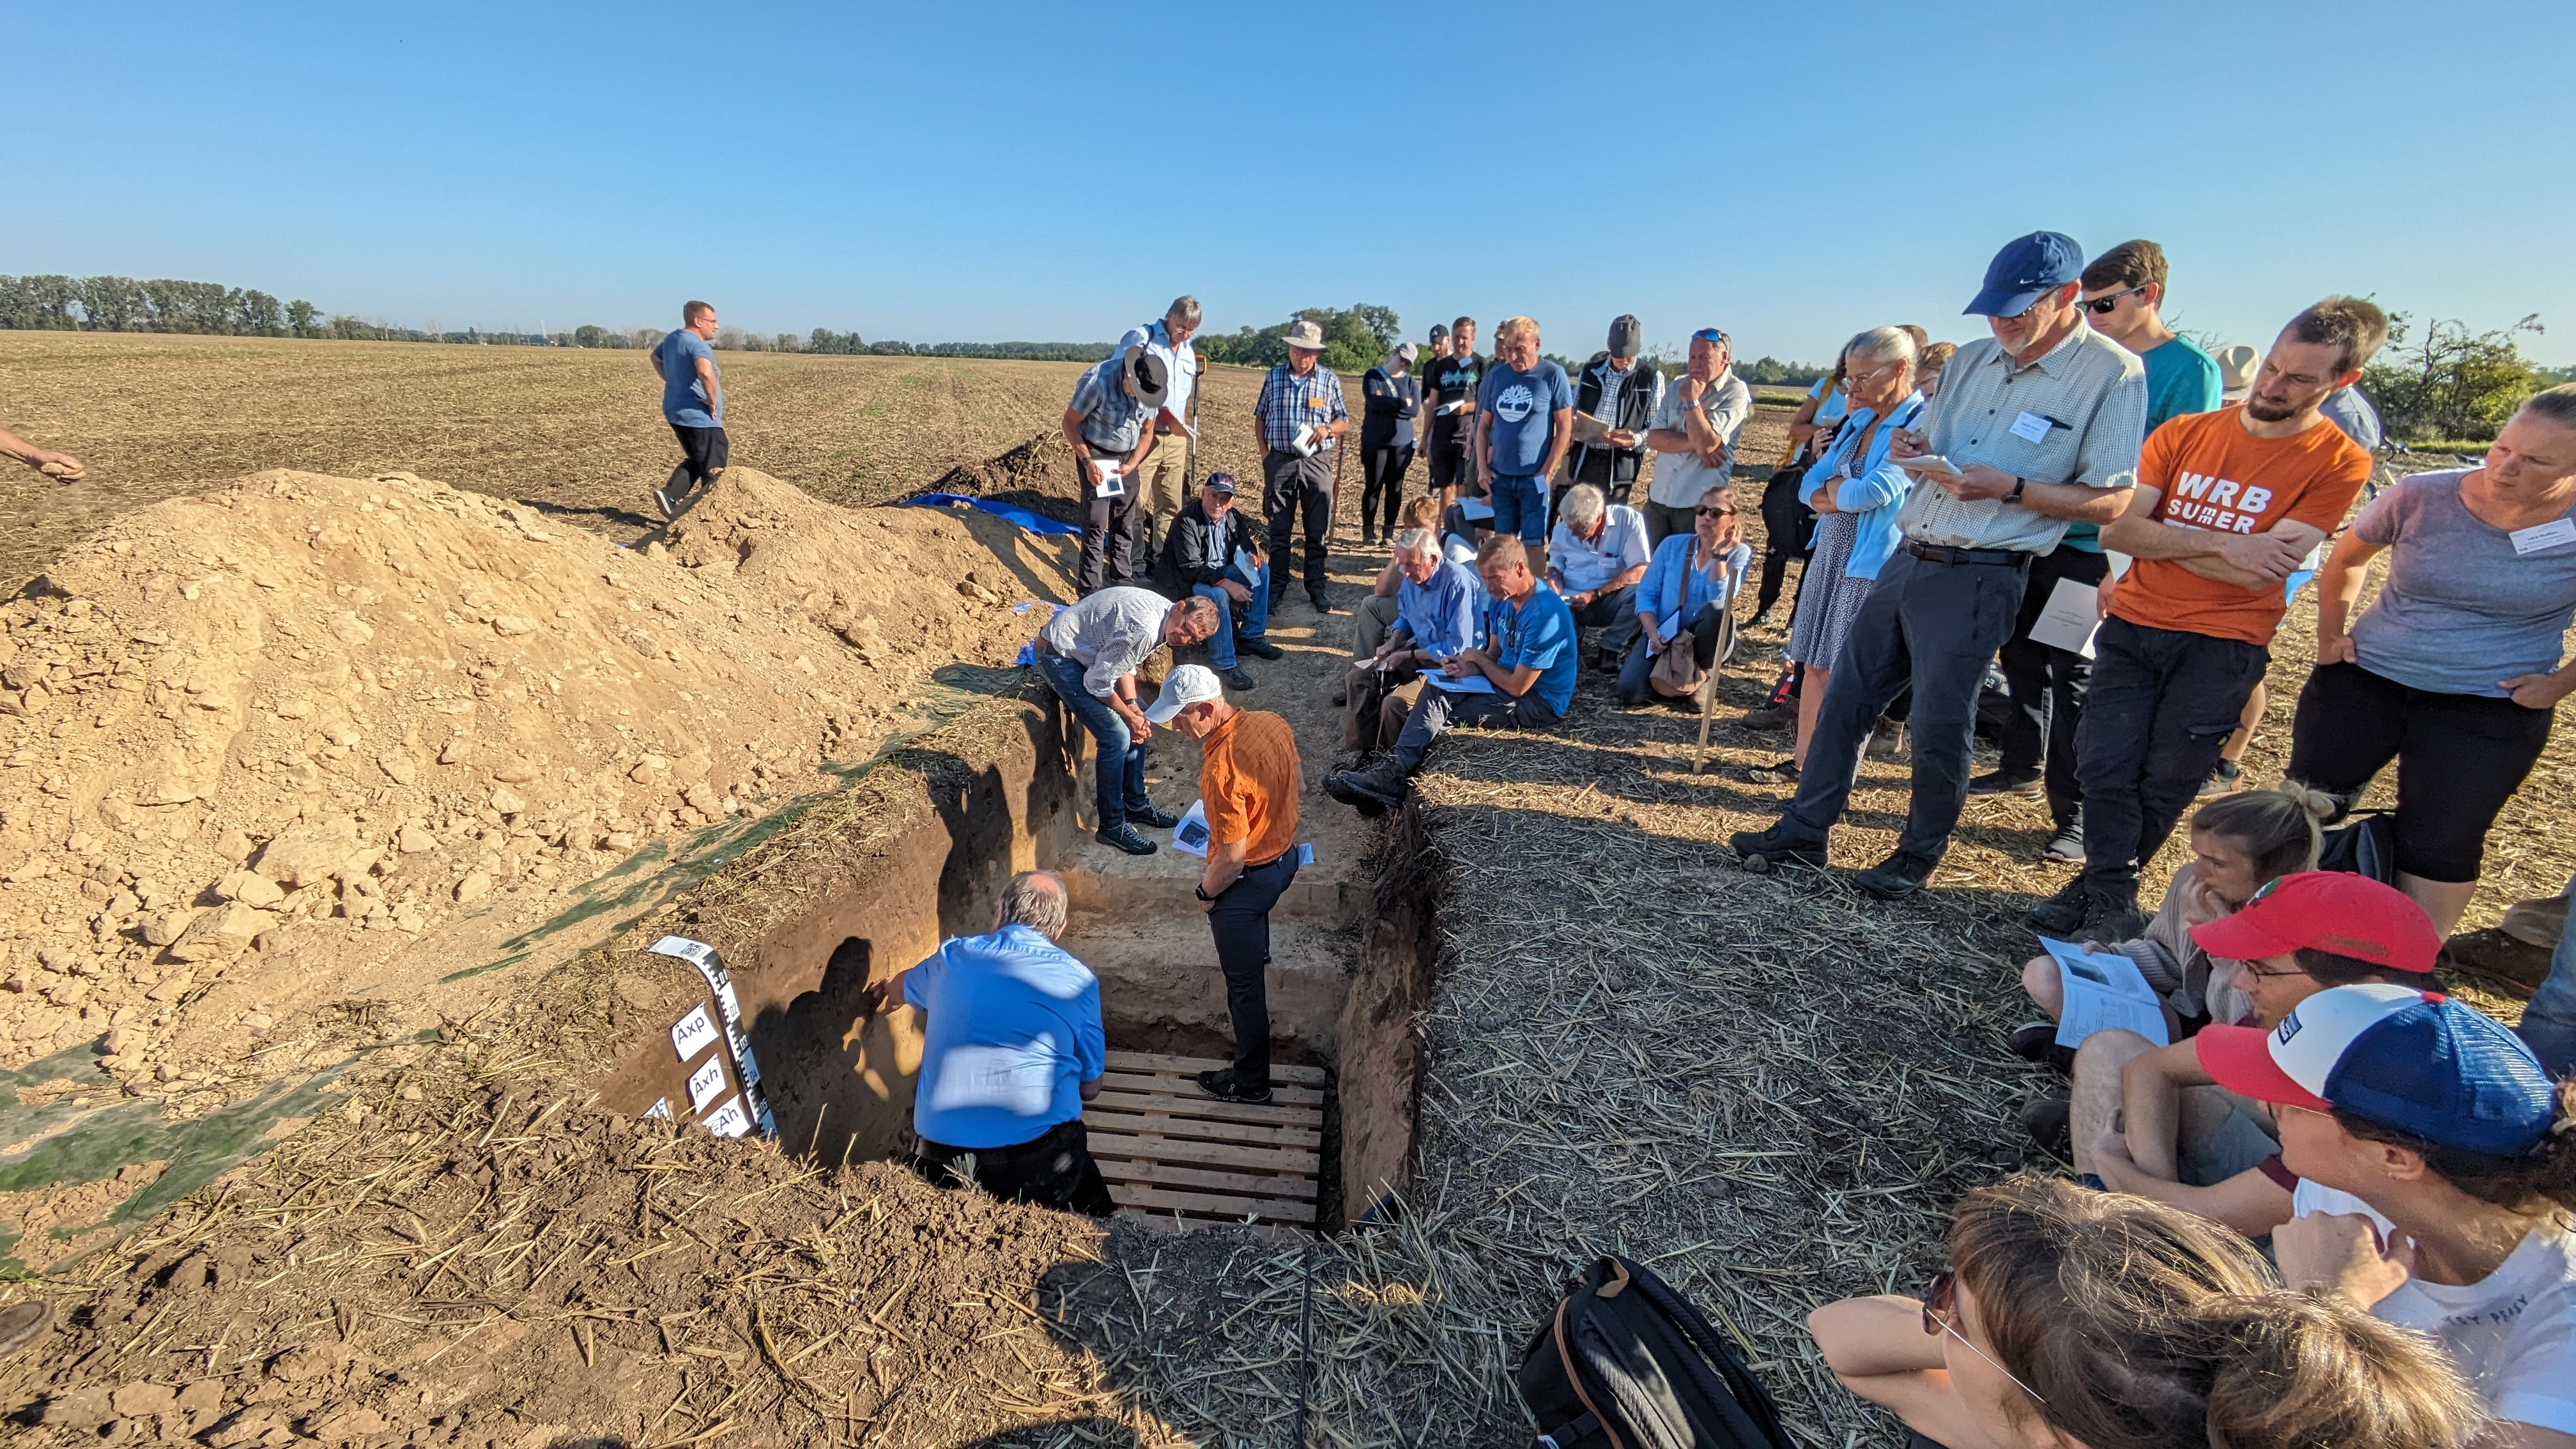
\includegraphics[width=1\textwidth]{FIGURE/PXL_20230908_074303007MP}
\end{block}
\end{frame}

%%%%%%%%%%%%%%%%%%%%%%%%%%%%%%%%%%%%%%%%%%%%%%%%%%%%%%%%%%%%%%%%%%%%%%%%%%%%%%%%%%%%%%%

\begin{frame}{Motivation}
\begin{block}{}
\centering\includegraphics[width=1\textwidth]{FIGURE/Scan_20230923_154907.jpg}
\end{block}
\end{frame}

%%%%%%%%%%%%%%%%%%%%%%%%%%%%%%%%%%%%%%%%%%%%%%%%%%%%%%%%%%%%%%%%%%%%%%%%%%%%%%%%%%%%%%%

\begin{frame}{Motivation}
\begin{columns}
\column{2.3cm}
\centering\includegraphics[width=1\textwidth]{FIGURE/Musterstueck.jpg} 

%\alert{TTn:p-eu}
 \column{9cm} 
 \begin{block}{Bodenkartierung}
\centering\includegraphics[width=1\textwidth]{FIGURE/03_bodenentstehung_website_2013_0.jpg}
\raggedright\tiny 
UBA, 2010. Die Böden Deutschlands -- Sehen, Erkunden, Verstehen. Umweltbundesamt.
\end{block}
\end{columns}
\end{frame}

%%%%%%%%%%%%%%%%%%%%%%%%%%%%%%%%%%%%%%%%%%%%%%%%%%%%%%%%%%%%%%%%%%%%%%%%%%%%%%%%%%%%%%%


\begin{frame}{Motivation}
 \begin{block}{Bodenkartierung}
\centering\includegraphics[width=0.95\textwidth]{FIGURE/Schwarzerden_LBGR.pdf}
 \end{block}
\raggedright\tiny\url{https://www.bodensystematik.de}
\end{frame}


%%%%%%%%%%%%%%%%%%%%%%%%%%%%%%%%%%%%%%%%%%%%%%%%%%%%%%%%%%%%%%%%%%%%%%%%%%%%%%%%%%%%%%%


\begin{frame}{Motivation}
\begin{columns}
\column{8.5cm}
\begin{block}{Bodenkartierung}
\centering\includegraphics[width=1\textwidth]{FIGURE/Scan_20230923_203922.pdf}
 \end{block}
 \column{2.5cm}
\raggedright\tiny Ad-hoc-Arbeitsgruppe Boden, 2005. Bodenkundliche Kartieranleitung, 5.Auflage. Schweizerbart’sche Verlagsbuchhandlung (Nägele und Obermiller), Stuttgart.
\end{columns}
\end{frame}




%%%%%%%%%%%%%%%%%%%%%%%%%%%%%%%%%%%%%%%%%%%%%%%%%%%%%%%%%%%%%%%%%%%%%%%%%%%%%%%%%%%%%%%


\begin{frame}{Motivation}

 \begin{block}{Bodenkartierung}
\centering\includegraphics[width=1\textwidth]{FIGURE/SoilMapping.png}
\end{block}
\raggedright\tiny 
Hengl, T., MacMillan, R.A., 2019. Predictive Soil Mapping with R. OpenGeoHub foundation, Wageningen.
\url{https://www.soilmapper.org}, ISBN: 978-0-359-30635-0     
\end{frame}

%%%%%%%%%%%%%%%%%%%%%%%%%%%%%%%%%%%%%%%%%%%%%%%%%%%%%%%%%%%%%%%%%%%%%%%%%%%%%%%%%%%%%%%

%\begin{frame}{Explainable Machine Learning}
%\begin{block}{Transparency, interpretability \& explainability}
%\centering\includegraphics[width=1\textwidth]{FIGURE/Explainability2.pdf} 
%\end{block}
%\raggedright\tiny   
%\begin{inparaitem}
%    \item Roscher, R., Bohn, B., Duarte, M.F., Garcke, J., 2020. Explainable Machine Learning for Scientific Insights and Discoveries. IEEE Access 8, 42200–42216. \url{https://doi.org/10.1109/ACCESS.2020.2976199      }
%    \item Rentschler, T., 2021. Explainable machine learning in soil mapping: Peeking into the black box. \url{https://doi.org/10.15496/PUBLIKATION-57960       }
%\end{inparaitem}
%\end{frame}

%%%%%%%%%%%%%%%%%%%%%%%%%%%%%%%%%%%%%%%%%%%%%%%%%%%%%%%%%%%%%%%%%%%%%%%%%%%%%%%%%%%%%%%
\begin{frame}{Explainable Machine Learning}
\begin{block}{Feature engineering}
\centering\includegraphics[width=1\textwidth]{FIGURE/Explainability1.pdf} 
\end{block}

\raggedright\tiny   
\begin{inparaitem}
    \item Roscher, R., Bohn, B., Duarte, M.F., Garcke, J., 2020. Explainable Machine Learning for Scientific Insights and Discoveries. IEEE Access 8, 42200–42216. \url{https://doi.org/10.1109/ACCESS.2020.2976199       }
    \item Rentschler, T., 2021. Explainable machine learning in soil mapping: Peeking into the black box. \url{https://doi.org/10.15496/PUBLIKATION-57960        }
\end{inparaitem}
\end{frame}

%%%%%%%%%%%%%%%%%%%%%%%%%%%%%%%%%%%%%%%%%%%%%%%%%%%%%%%%%%%%%%%%%%%%%%%%%%%%%%%%%%%%%%%
\begin{frame}{Explainable Machine Learning}

\begin{block}{}
\alert{Transparency} considers the ML approach, \alert{interpretability} considers the ML model together with data, and \alert{explainability} considers the model, the data, and human involvement.
\end{block}

\begin{alertblock}{Feature engineering}
\begin{itemize}
    \item adjusting and reworking the predictors to enable models to better uncover predictor-response relationships
    \item the process of creating representations of data that increase the effectiveness of a model
\end{itemize}
\end{alertblock}




\raggedright\tiny  
\begin{inparaitem}
\item Roscher, R., Bohn, B., Duarte, M.F., Garcke, J., 2020. Explainable Machine Learning for Scientific Insights and Discoveries. IEEE Access 8, 42200–42216. \url{https://doi.org/10.1109/ACCESS.2020.2976199     }
\item Kuhn, M., Johnson, K., 2019. Feature Engineering and Selection: A Practical Approach for Predictive Models, 1st ed. Chapman and Hall/CRC. \url{https://doi.org/10.1201/9781315108230     }
\end{inparaitem}
\end{frame}



%%%%%%%%%%%%%%%%%%%%%%%%%%%%%%%%%%%%%%%%%%%%%%%%%%%%%%%%%%%%%%%%%%%%%%%%%%%%%%%%%%%%%%%
\begin{frame}{Explainable Machine Learning}
\begin{block}{Feature engineering}
\centering\includegraphics[width=1\textwidth]{FIGURE/Figure_Flowchart2-KoBoS.pdf}
\end{block}

\begin{columns}
    \column{8cm}
    \raggedright\tiny  Möller, M., Zepp, S., Wiesmeier, M., Gerighausen, H., Heiden, U., 2022. Scale-Specific Prediction of Topsoil Organic Carbon Contents Using Terrain Attributes and SCMaP Soil Reflectance Composites. Remote Sensing 14, 2295. \url{https://doi.org/10.3390/rs14102295        }
    \column{3cm}
\href{https://github.com/FLFgit/ScaleP/wiki}{\centering\includegraphics[width=0.5\textwidth]{FIGURE/Github.png}}\\
\href{https://zenodo.org/record/7895529}{\centering\includegraphics[width=1\textwidth]{FIGURE/Zenodo.png}}
\end{columns}
\end{frame}

%%%%%%%%%%%%%%%%%%%%%%%%%%%%%%%%%%%%%%%%%%%%%%%%%%%%%%%%%%%%%%%%%%%%%%%%%%%%%%%%%%%%%%%

%\begin{frame}{Feature engineering: \alert{Scale}}
%\begin{columns}
% \column{5.45cm}
% \begin{block}{}
% \centering\includegraphics[width=1\textwidth]{FIGURE/Figure_Segmentation1.png}
%\end{block}
% \column{4.5cm}
% \begin{block}{}
% \centering\includegraphics[width=1\textwidth]{FIGURE/Figure_Segmentation2.png}
% \end{block}
%  \end{columns}
%\raggedright\tiny 
%\vspace{4,9pt}
%\begin{inparaitem}
%     \item Möller M, Koschitzki T, Hartmann K-J, Jahn R. Plausibility test of conceptual soil maps using relief parameters. CATENA 2012;88:57–67. \url{https://doi.org/10.1016/j.catena.2011.08.002}     .
%     \item  Möller M, Volk M. Effective map scales for soil transport processes and related process domains — Statistical and spatial characterization of their scale-specific inaccuracies. Geoderma 2015;247–248:151–60. \url{https://doi.org/10.1016/j        .geoderma.2015.02.003}.
%     \item  Möller M, Volk M, Friedrich K, Lymburner L. Placing soil-genesis and transport processes into a landscape context: A multiscale terrain-analysis approach. J Plant Nutr Soil Sci 2008;171:419–30. \url{https://doi.org/10.1002/jpln.200625039}    .
% \end{inparaitem}
%\end{frame}

%%%%%%%%%%%%%%%%%%%%%%%%%%%%%%%%%%%%%%%%%%%%%%%%%%%%%%%%%%%%%%%%%%%%%%%%%%%%%%%%%%%%%%%
\begin{frame}{Feature engineering: \alert{Scale}}
\begin{columns}
 \column{5cm}
 \begin{block}{Topographic Position Index}
\centering\includegraphics[width=1\textwidth]{FIGURE/TPI.png}
\end{block}

\raggedright\tiny Guisan, A., Weiss, S.B., Weiss, A.D., 1999. GLM versus CCA spatial modeling of plant species distribution. Plant Ecology 143, 107–122. \url{https://doi.org/10.1023/A:1009841519580    }

\column{5cm}
\centering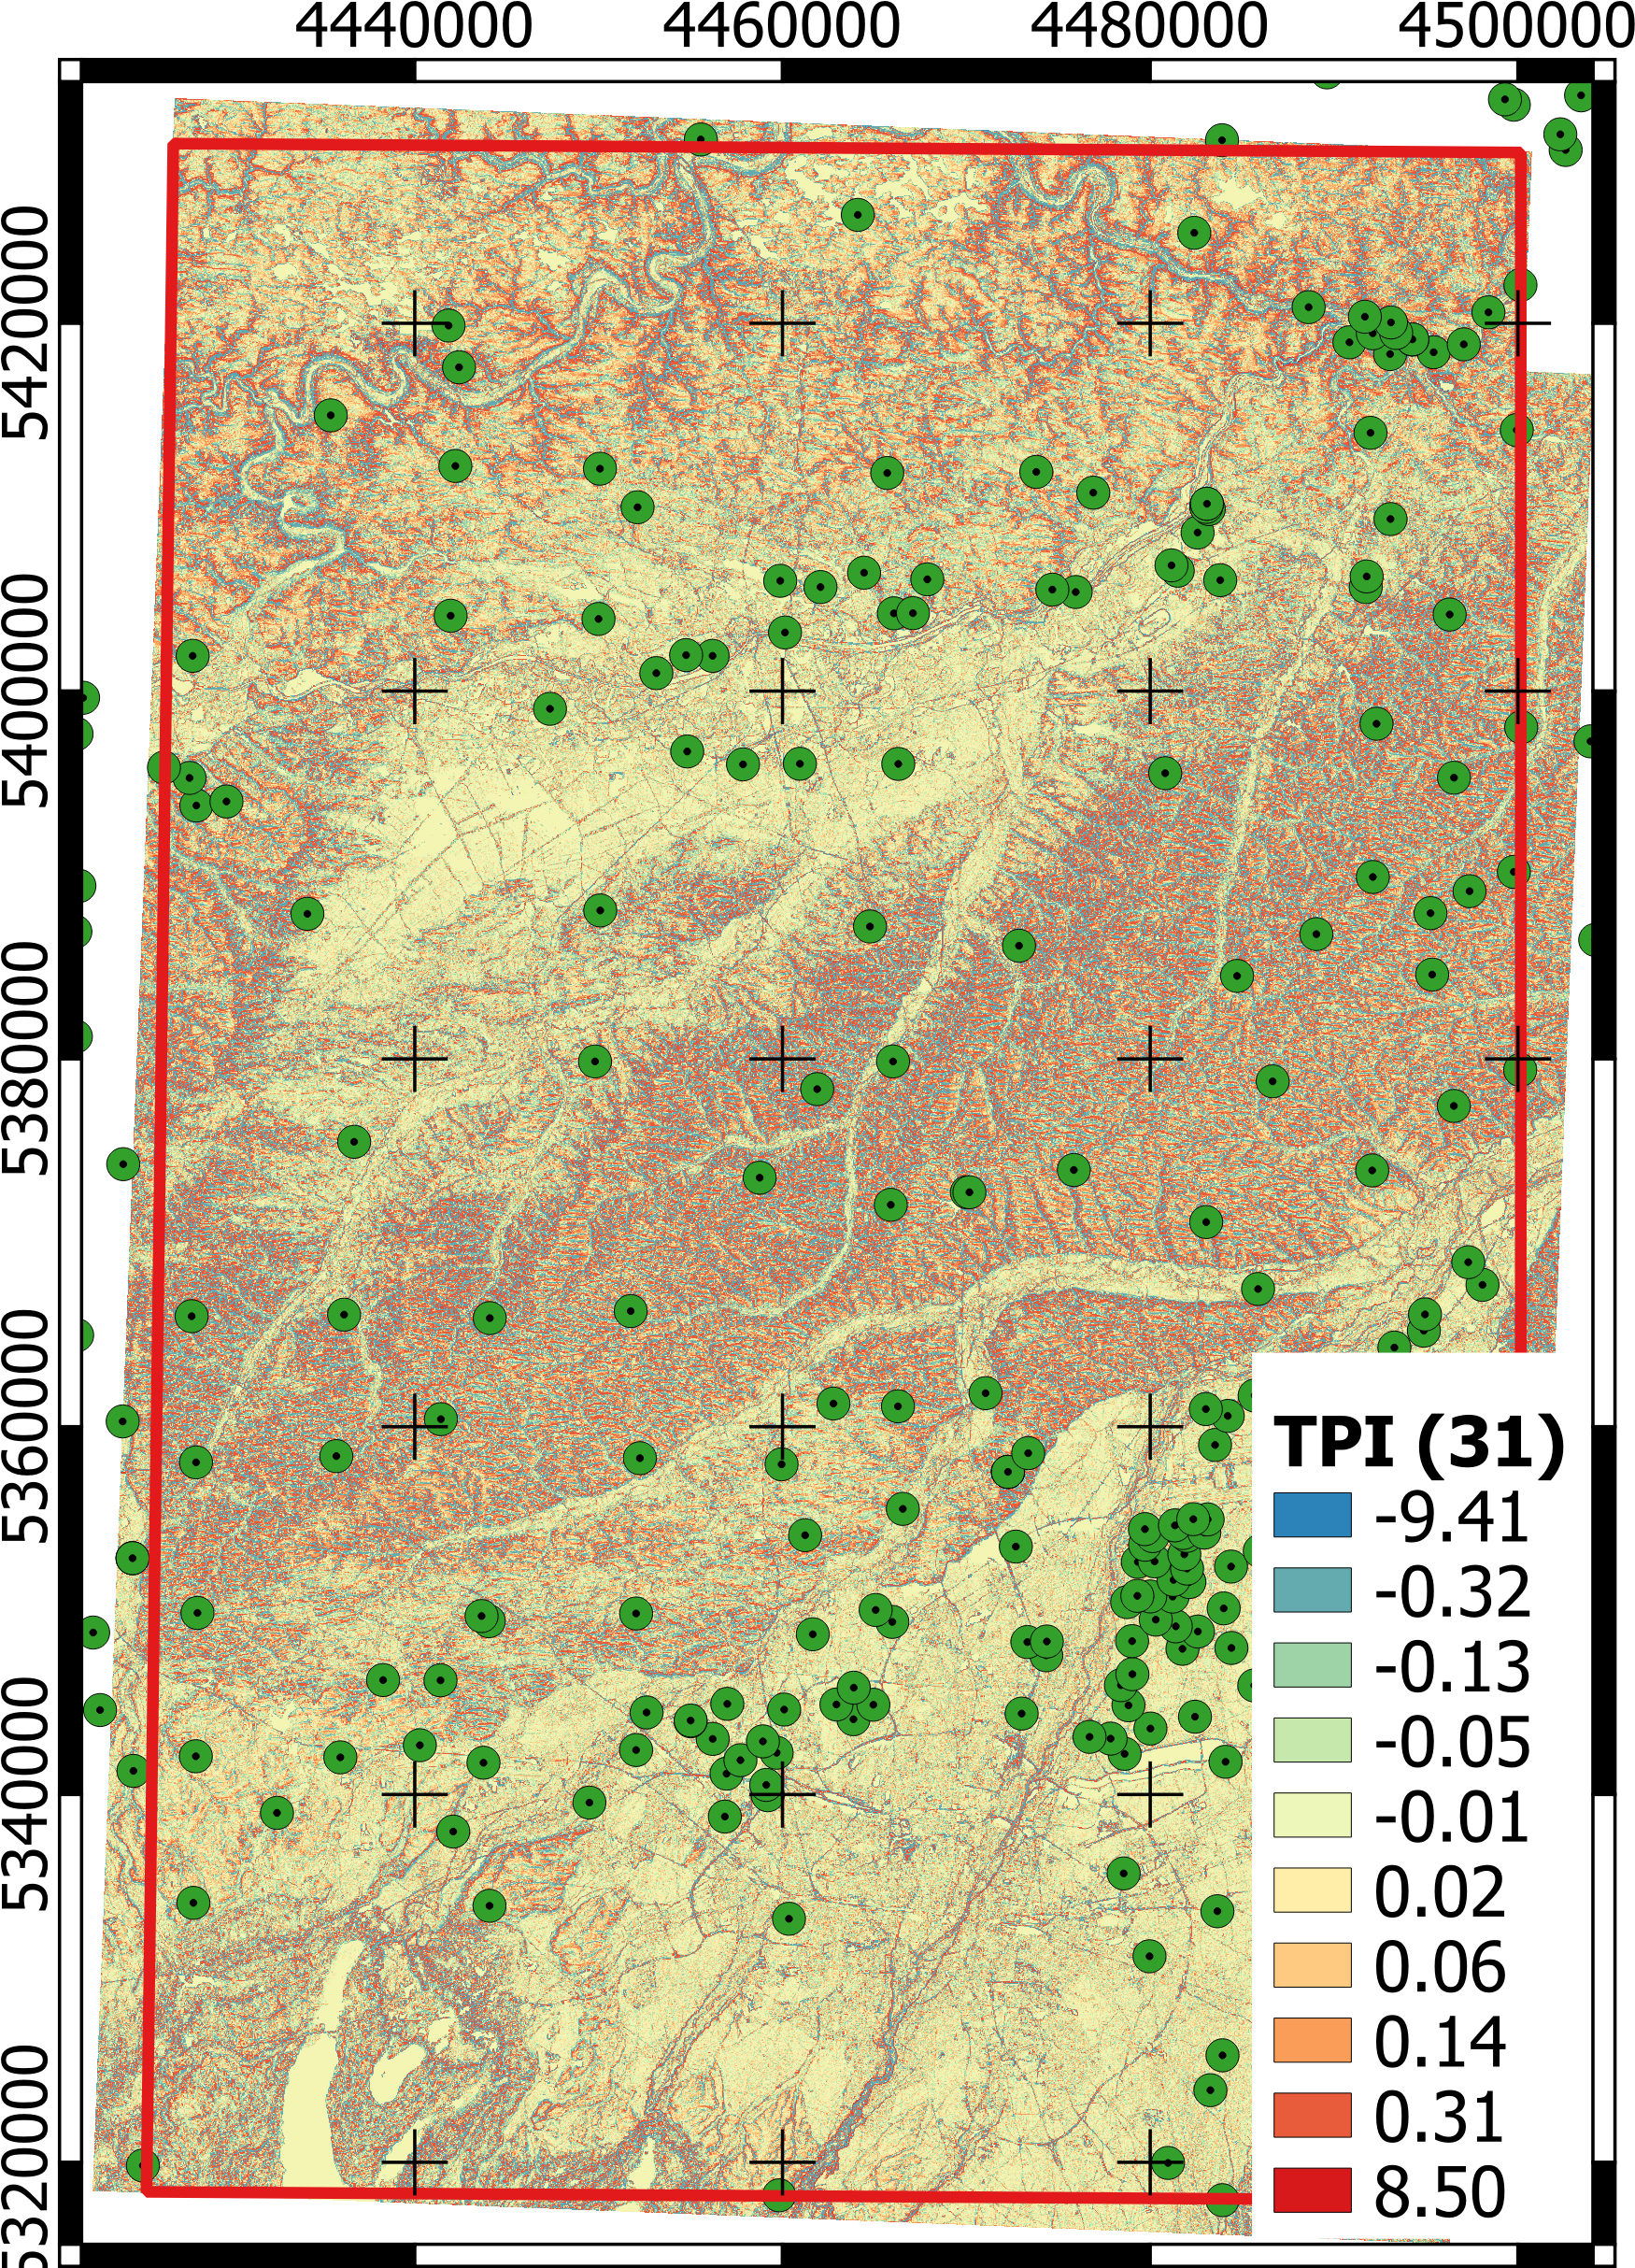
\includegraphics[width=1\textwidth]{FIGURE/TPI32.png}

\end{columns}
\end{frame}

%%%%%%%%%%%%%%%%%%%%%%%%%%%%%%%%%%%%%%%%%%%%%%%%%%%%%%%%%%%%%%%%%%%%%%%%%%%%%%%%%%%%%%%
\begin{frame}{Feature engineering: \alert{Scale}}
\begin{columns}
 \column{5cm}
 \begin{block}{Topographic Position Index}
\centering\includegraphics[width=1\textwidth]{FIGURE/TPI.png}
\end{block}

\raggedright\tiny Guisan, A., Weiss, S.B., Weiss, A.D., 1999. GLM versus CCA spatial modeling of plant species distribution. Plant Ecology 143, 107–122. \url{https://doi.org/10.1023/A:1009841519580   }

\column{5cm}
\centering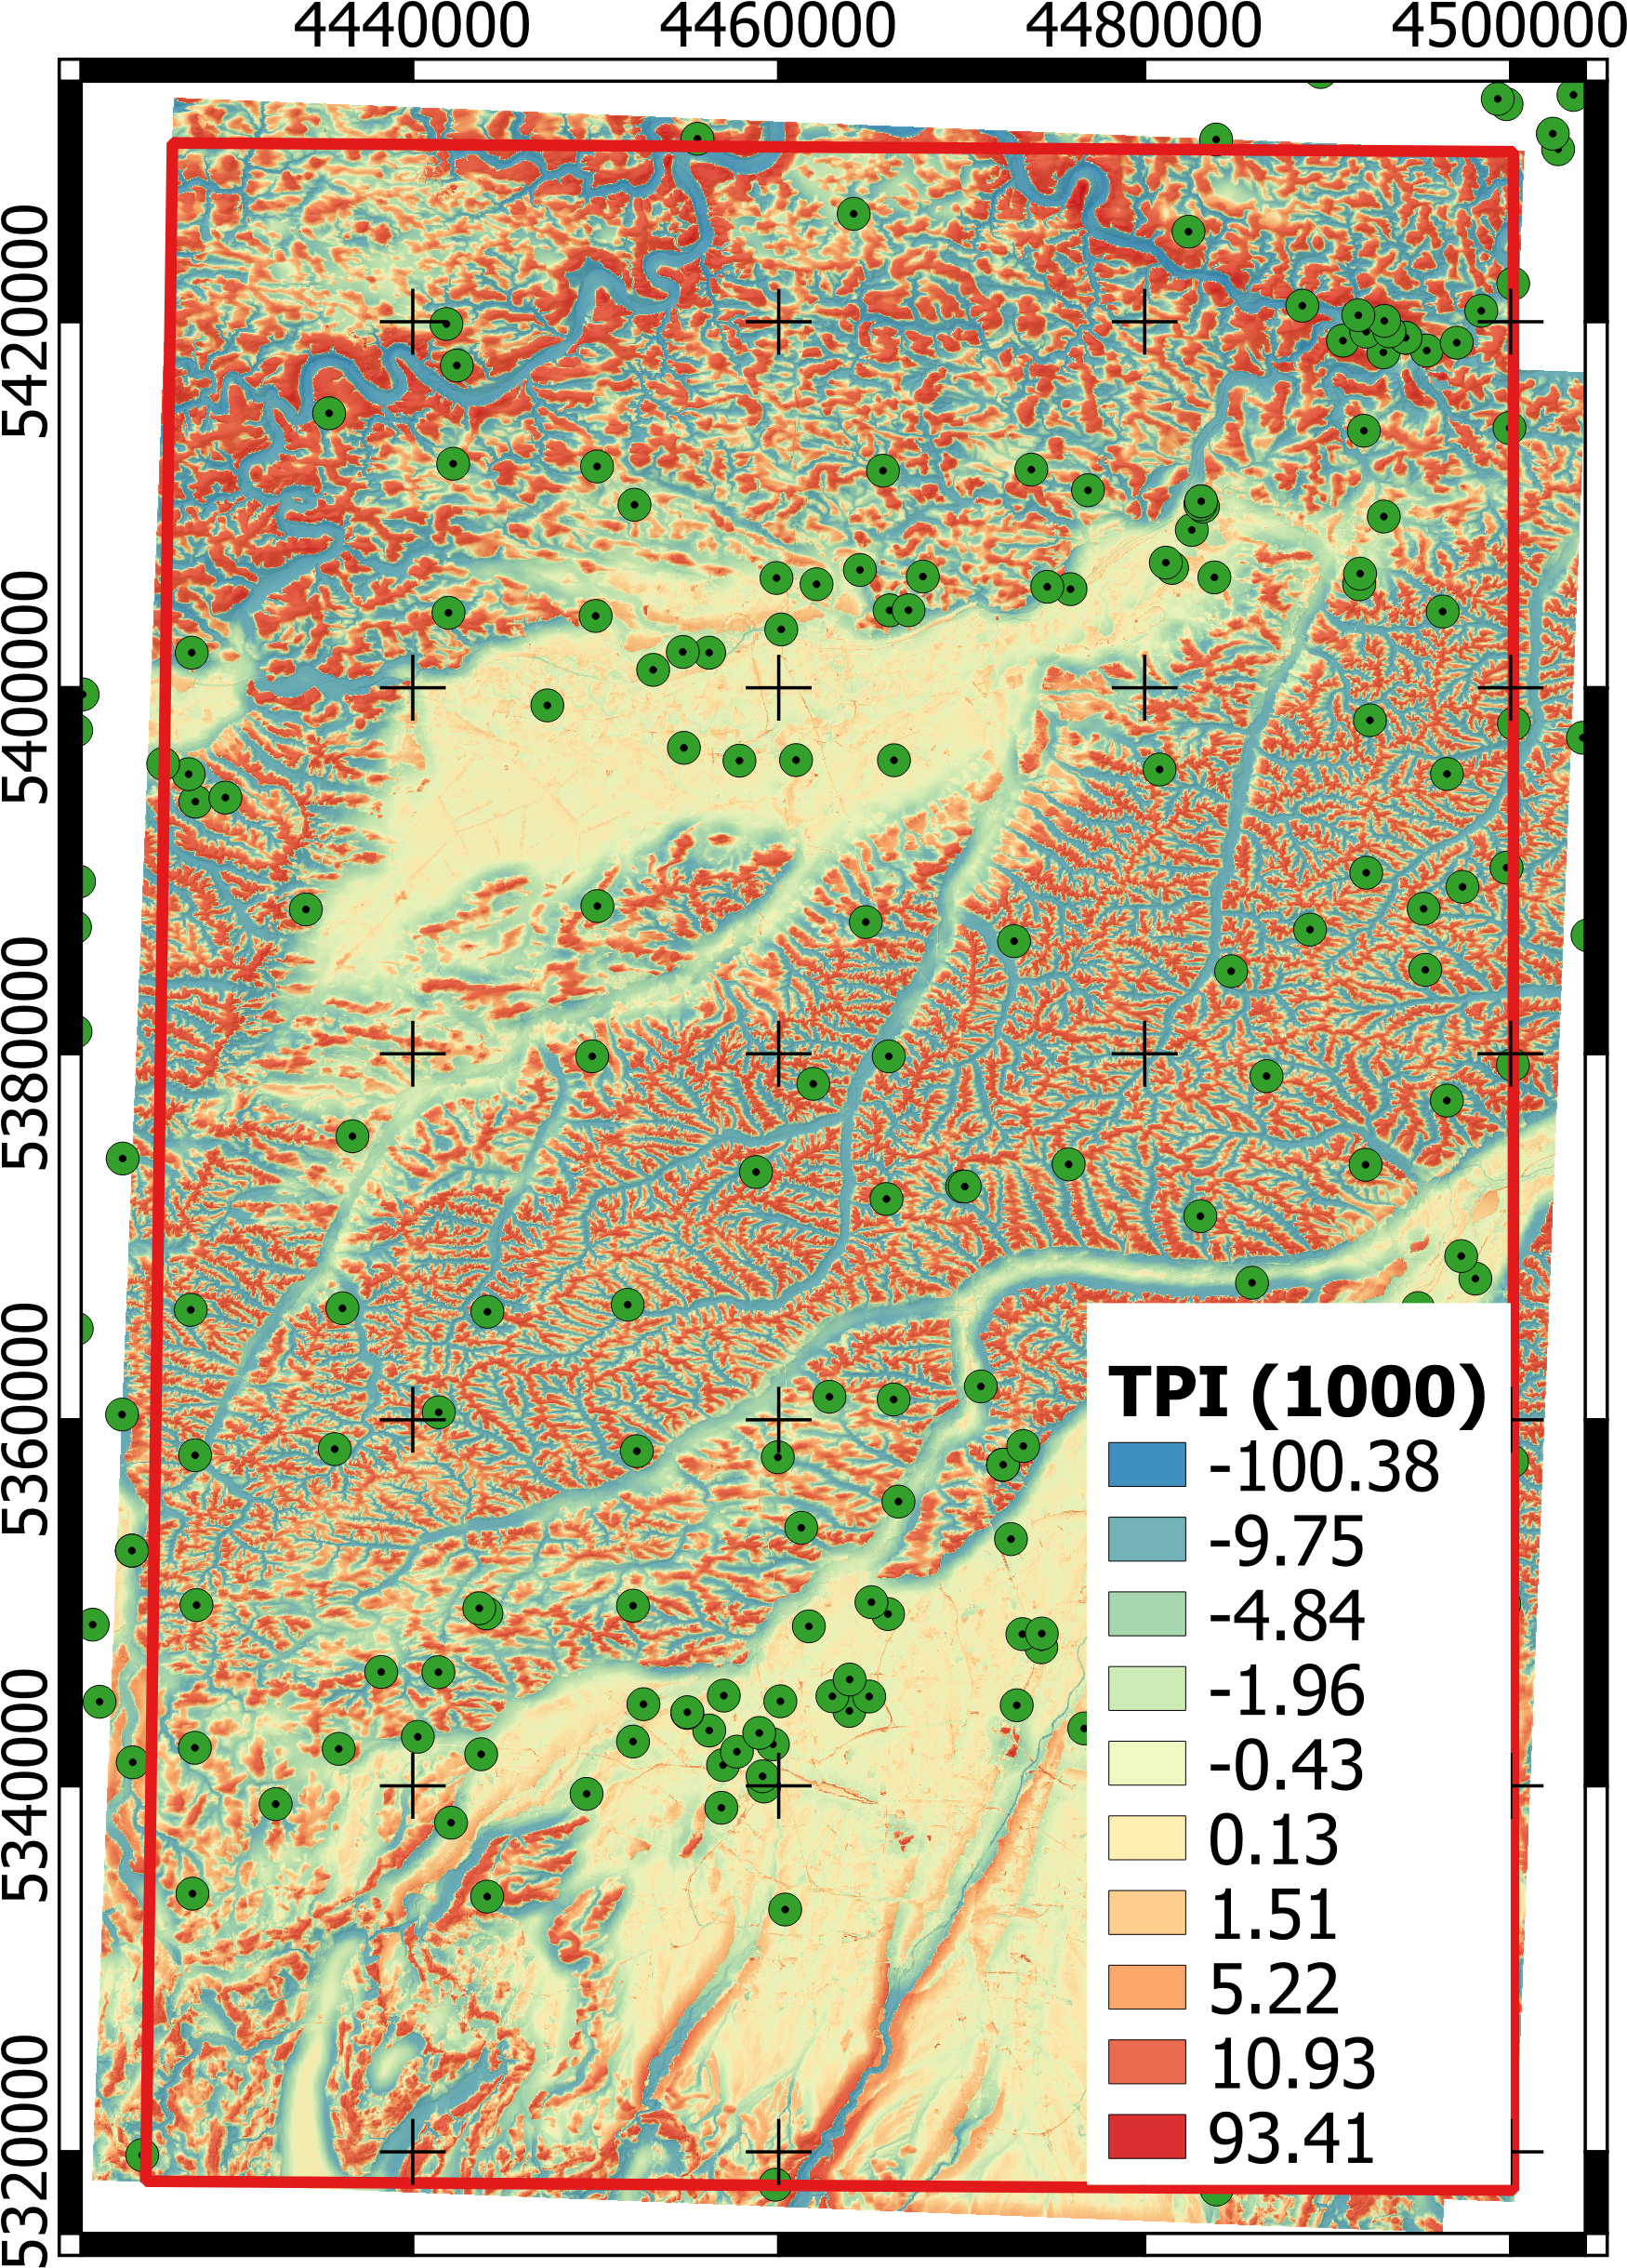
\includegraphics[width=1\textwidth]{FIGURE/TPI1000.png}

\end{columns}
\end{frame}

%%%%%%%%%%%%%%%%%%%%%%%%%%%%%%%%%%%%%%%%%%%%%%%%%%%%%%%%%%%%%%%%%%%%%%%%%%%%%%%%%%%%%%%
\begin{frame}{Feature engineering: \alert{Time}}
\begin{columns}
 \column{8cm}
 \begin{block}{Bodenreflektanzkomposite (SCMaP-SRC)}
\centering\includegraphics[width=1\textwidth]{FIGURE/BareSoilIndex.pdf}

\raggedright\tiny https://www.soil-de.eomap.de
\end{block}
 \column{3cm}

\raggedright\tiny 
\begin{inparaitem}
    \item Rogge, D., Bauer, A., Zeidler, J., Mueller, A., Esch, T., Heiden, U., 2018. Building an exposed soil composite processor (SCMaP) for mapping spatial and temporal characteristics of soils with Landsat imagery (1984–2014). Remote Sensing of Environment 205, 1–17. \url{https://doi.org/10.1016/j.rse.2017.11.004      }
    \item Zepp, S., Heiden, U., Bachmann, M., Möller, M., Wiesmeier, M., van Wesemael, B., 2023. Optimized Bare Soil Compositing for Soil Organic Carbon Prediction of Topsoil Croplands in Bavaria using Landsat. ISPRS Journal of Photogrammetry and Remote Sensing 202, 287-302. \url{https://doi.org/10.1016/j.isprsjprs.2023.06.003         } 
\end{inparaitem}

\end{columns}
\end{frame}




\begin{frame}{Zusammenfassung und Ausblick}
\begin{alertblock}{Feature engineering $\dots$}
\begin{itemize}
\item formalisiert Experten- und Domainwissen,
\item erhöht die Modellgüte und -akzeptanz.
\end{itemize}
\end{alertblock}
\pause
\begin{block}{\href{https://wissen.julius-kuehn.de/klimaschutz/projekte/erhoehung-kohlenstoffspeicherpotentiale/kobos}{KoBoS}}
Deutschlandweite raum-zeitliche Modellierung von \textcolor{red}{Ko}hlenstoffgehalten
landwirtschaftlicher \textcolor{red}{Bö}den durch eine integrative Auswertung von
\textcolor{red}{S}atellitenbildzeitreihen und Geodaten (\textcolor{red}{KoBoS})
\begin{itemize}
    \item Bereitstellung von Webdiensten deutschlandweit erklärender erklärenden Variablen nach FAIR-Prinzipien,
    \item Entwicklung eines erweiterbaren, dynamischen und webbasierten Open-Source-Modells, das für beliebige Gebiete in Deutschland anwendbar ist.
    \end{itemize}

\tiny gefördert durch das BMEL-Klimaschutz-Sofortprogramm 2022 $|$ \#RessortForschtKlima $|$ \url{https://wissen.julius-kuehn.de/klimaschutz/projekte/erhoehung-kohlenstoffspeicherpotentiale/kobos}
\end{block}


\end{frame}

%\begin{frame}{Ausblick}

%\begin{block}{Feature engineering}
%\begin{inparaitem}
%     \item Möller M, Koschitzki T, Hartmann K-J, Jahn R., 2012, Plausibility test of conceptual soil maps using relief parameters. CATENA 2012;88:57–67. https://doi.org/10.1016/j              .catena.2011.08.002.
%     \item  Möller M, Volk M., 2015, Effective map scales for soil transport processes and related process domains — Statistical and spatial characterization of their scale-specific inaccuracies. Geoderma 2015;247–248:151–60. https://doi.org/10.1016/j                  .geoderma.2015.02.003.
%     \item  Möller M, Volk M, Friedrich K, Lymburner L., 2008, Placing soil-genesis and transport processes into a landscape context: A multiscale terrain-analysis approach. Journal of  Plant Nutrion and Soil Science, 171:419–30. https://doi.org/10.1002/jpln.200625039       .
% \end{inparaitem}
%\end{block}
%\end{frame}




\begin{frame}{\alert{Fragen?}}
 \centering\includegraphics[width=1\textwidth]{FIGURE/big_cover-remotesensing-v14-i10.png}     
\end{frame}

\end{document}


